\chapter{ Le vademecum du Modèle Standard }
\renewcommand\chapterillustration{SM/sm2}
\ThisULCornerWallPaper{1}{\chapterillustration}
\minitoc

\lettrine[lines=4, slope=-0.5em]{D}{ans} ce chapitre, un bref historique de la Physique des particules est donné ainsi qu'un résumé et une description de la théorie la plus aboutit dans ce domaine, appellée le Modèle Standard (MS). Il sera également discuté des faiblesse et limites de cette théorie ainsi que de ses éventuelles extensions.

\section{Un bref historique}

\marginpar
{
\begin{center}
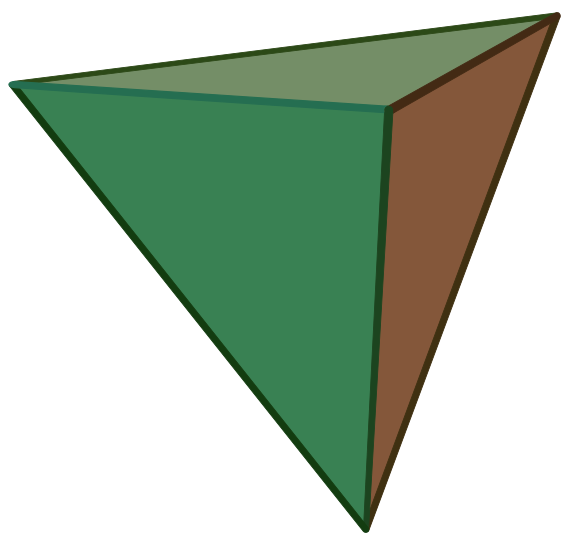
\includegraphics[width=0.25\marginparwidth]{SM/Tetrahedron.png}
\vspace*{-0.25cm}
\begin{center}\normalfont\small {Le Tétraèdre (le Feu).}\end{center}
\vspace*{-0.25cm}
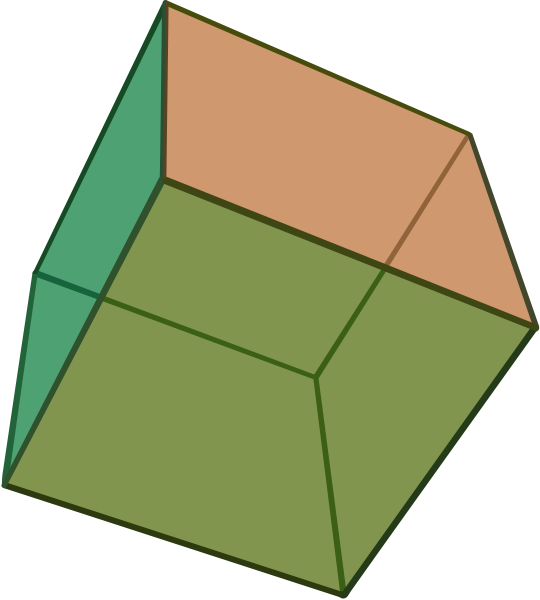
\includegraphics[width=0.25\marginparwidth]{SM/Hexahedron.png}
\vspace*{-0.25cm}
\begin{center}\normalfont\small {Le Cube (la Terre).}\end{center}
\vspace*{-0.25cm}
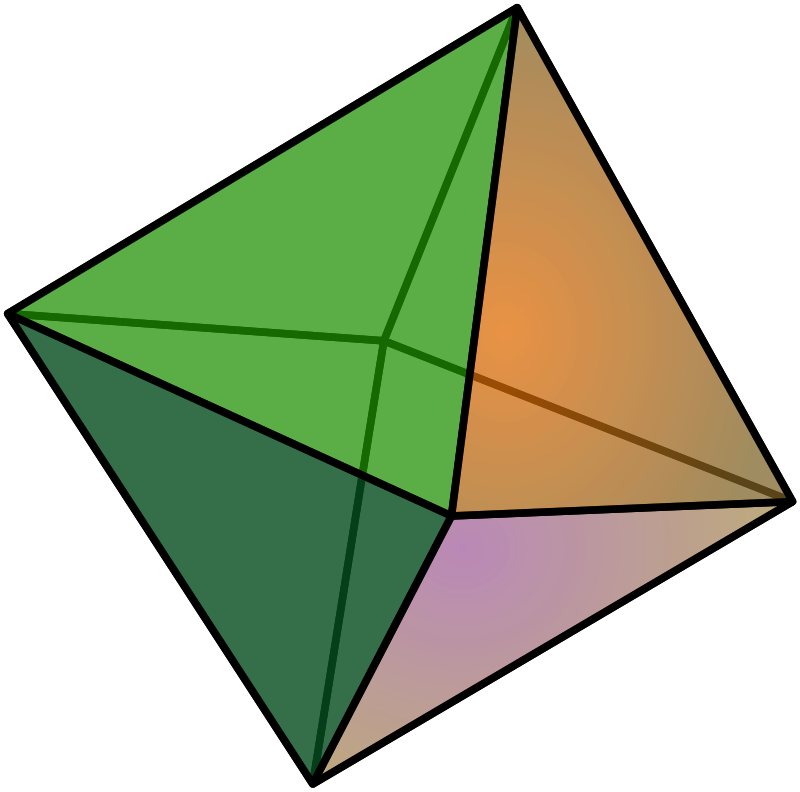
\includegraphics[width=0.25\marginparwidth]{SM/Octahedron.png}
\vspace*{-0.25cm}
\begin{center}\normalfont\small {L'Octaèdre (l'Air).}\end{center}
\vspace*{-0.25cm}
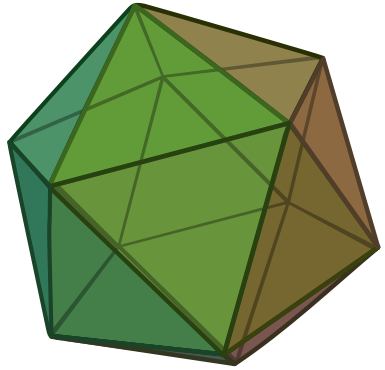
\includegraphics[width=0.25\marginparwidth]{SM/Icosahedron.png}
\vspace*{-0.25cm}
\begin{center}\normalfont\small {L'Icosaèdre (l'Eau).}\end{center}
\vspace*{-0.25cm}
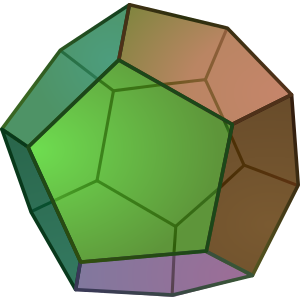
\includegraphics[width=0.25\marginparwidth]{SM/Dodecahedron.png}
\vspace*{-0.25cm}
\begin{center}\normalfont\small {Le Dodécaèdre (l'Univers).}\end{center}
\vspace*{-0.25cm}
\captionof{figure}{Les solides de Platon.}
\label{solides}
\end{center}
}
De tout temps les hommes ont voulu comprendre et maitriser la nature. Cette quête à amener de nombreux penseurs, et notamment les philosophes Grecs, à proposer des explications sur le monde qui nous entoure, et certaines de leurs idées se révélerons florisantes et donneront naissances des siècles plus tard à la naissance de la Physique en tant que science au sens moderne du mot. 

Anaxagore (~500-428 av. J.C.) pronait que toute chose est formée de particules élementaires. Cette idée sera reprise par Empédocle (~495-~435 av J.C) qui proposa, l'eau, la terre, l'air et le feu comme étant ces particules. Platon (428/427 - 348/347 av. J.C.) associera ces quatres éléménts aux polygones réguliers convexes de l'espace à trois dimension (le tétraèdre pour le Feu, le cube pour la Terre, l'octaèdre pour l'Air, l'icosaèdre pour l'Eau, le dodécaère reprèsente l'éther, élément constituant l'Univers (fig.\ref{solides})). On doit à Leucippe (~460-~370 av J.C.) et son disciple Démocrite (~460-~370 av J.C.) le concept d'atome qui compose la matière et est indivisible et séparés par du vide. La véracité de l'atomisme fera débat pendant des siècles et ne sera validé expérimentalement qu'au cours du XIX\ieme siècle.

 Parmis les travaux les plus importants qui prouverons l'existence des atomes, citons ceux de Lavoisier (1743-1794) qui décompose de nombreuses substances en "Éléments". De nombreux travaux sur les gaz, la cristallographie, la physique statistique et la thermodynamique : Bernouilli (1700-1782) : cinétique des gaz, Haüy (1743-1822) : La forme des cristaux reflète la symétrie des "briques élémentaire" le constituant , Dalton (1766-1844) : symbolisation des corps simples et des corps composés par des symboles auxquels il donne un poids de matière (fig.\ref{atom}), et liste des masses atomiques d'un certain nombre d'éléments rapportés à la masse de l'hydrogène, Gay-Lussac (1778-1850) : les rapports des volumes des réactifs et des produits de réaction sont des nombres entiers petits , Maxwell(1831-1879) : dispersion statistique des vitesses des molécules, Boltzmann (1844-1906) : répartition statistique des vitesses dans un gaz , Mendeleïev : Classification périodique des éléments et prédiction de nouveaux atomes (fig.\ref{periodique}).Ces travaux ferons passer petit à petit cet théorie en réalité scientifique. 
 
\marginpar
{
	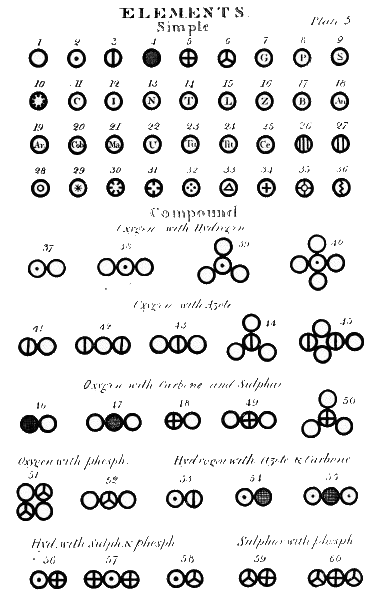
\includegraphics[width=\marginparwidth]{SM/Dalton.png}
    \captionof{figure}{Dessins de divers atomes et molécules tirés de l'ouvrage \textit{A New System of Chemical Philosophy}}
    	\label{atom}
}
\marginpar
{
	\vspace{2cm}
		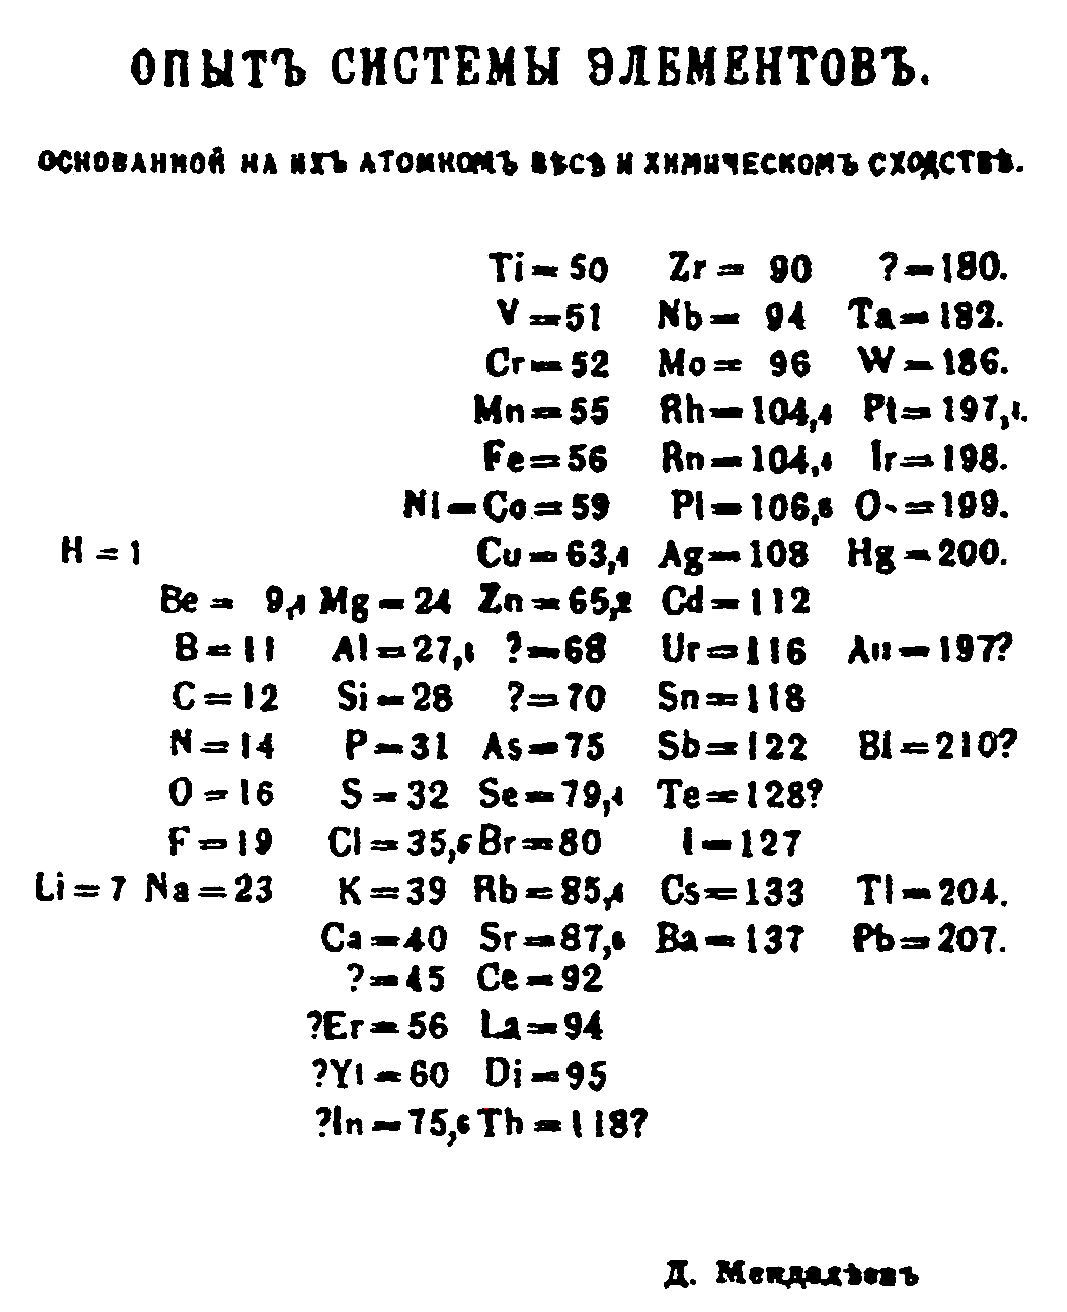
\includegraphics[width=\marginparwidth]{SM/periodique.png}
    \captionof{figure}{Tableau périodique de Mendeleïev}
    	\label{periodique}
}
D'autres domaine de la Physique connaitront des bouleversement important au cours des siècles : 

Pour la Mécanique et la cosmologie : Copernic (1473-1543) et Galilée (1564-1642) : Modèle héliocentique, Tycho Brahe (1546-1601) : remise en cause de  l'immuabilité du monde supra-lunaire énoncée par Aristote, Kepler (1571-1630) : Orbite elliptique des planètes, Newton (1643-1727) : théorie de la gravitation universelle, Lagrange (1736-1813) et Hamilton (1805-1865) : Principe de moindre action, Lagrangien, Hamiltonien.

Pour l'électromagnètisme : Coulomb(1736-1806) : loi de Coulomb, Volta(1745-1827): pile voltaïque, Ørsted (1777-1851), Ampère(1775-1836), Faraday(1792-1867), Henry (1797-1878) : les phénomènes d'inductions, Maxwell : Équations de Maxwell.

Avec la découverte de l'électron par Thomson (1856-1940) en 1887 qui fût prédit en 1874 par Laming et Stoney. Thomson développe le premier modèle de l'atome, qui est décrit comme une boule de charge neutre possédant un noyau positif avec des électrons négatifs (modèle de plum-pudding). On découvre également durant cette période la radioactivité (Becquerel (1852-1908)). La physique semble à cette époque complète et cohérente. Lord Kelvin dira même dans son discourt à la "Royal Instution of Great Britain" : \textit{"The beauty and clearness of the dynamical theory, which asserts heat and light to be modes of motion, is at present obscured by two clouds."}. Ces deux "nuages", l'incapacité à détecté l'éther luminifère  (expérience de Michelson-Morley) et la catastrophe ultaviollette du corps noir, donneront naissance respectivement à la relativité restreinte et à la mécanique quantique et feront entrer les physiciens dans la Physique Moderne.

Le début du siécle dernier sera une période florissante pour la physique des particules. Planck (1858-1947) afin de résoudre le problème du corps noir, proposera de quantifier les rayonnements : ceux-ci ne peuvent être qu'un multiple d'une constante qui porte son nom ($h$). Einstein ira plus loin est expliquera durant l'\textit{Annus mirabilis} (1905) l'effet photoélectrique en proposant le photon comme quanta de lumière qui agit comme une particule. Il possera également les bases de la relativité restreinte cette même année, réfutant le concept d'éther. De nombreux physicien vont ensuite poser les bases que la mécanique quantique: Bohr (1885-1962), Compton (1892-1962), De Broglie (1892-1987), Schrödinger (1887-1961), Heisenberg (1901-1976), Dirac (1902-1984), Pauli (1900-1958). Avec les progrés tant théorique qu'instrumentaux de Physiciens tels  Rutherford (1871-1937), Chadwick (1891-1974), Fermi (1901-1954), qui explore le monde subatomique; On découvre les deux forces agissant à l'échelle du subatomique (la force faible et forte) qui s'ajoute au deux force connu à l'époque (la force gravitationnelle et la force éléctromagnétique). Des physiciens tel Schwinger (1918-1994) veulent continuer la réunification des forces déjà avancée par les travaux de Maxwell ( force éléctrique et magnétique). Dans les année 1960, Weindberg (1933) et Salam (1926-1996) et Glashow (1932), réunissent dans une théorie dite électrofaible les forces électromagnétique et faible. Cette théorie prédit trois bosons ($W^{+}$, $W^{-}$ et $Z^{0}$). Leur théorie nécessite un boson suplémentaire, le boson de Higgs, postué en 1964 par Brout, Englert, Higgs, Haggen Guralnik et Kibble afin de donner une masse aux particules. Cette théorie est la base du Modèle Standard de la physique des particules. La découverte des quarks amène à la création de la Chromodynamique Quantique (QCD) par Politzer (1949), Wilczek (1951), Gross (1941) afin de décrire l'interaction forte. Elle sera ensuite intégrée au Modèle Standard.

À partir de la seconde moitiè du XX\ieme siècle, la Physique Subatomique à tâché à valider cette théorie et notament par la découverte des bosons  $W^{+}$,$W^{-}$ et $Z^{0}$ en 1983,le quarks top $t$ en 1995, neutino tauique en 2000 et du boson de Higgs $h$ en 2012. De nombreux efforts sont également mené afin de continuer l'unification des forces entre elles. On sait désormais que le Modèles Standard, bien que jamais mis en défaut, ne peut tout expliquer. Certaines questions reste ouvertes et cette théorie présente même quelques défaults. La technicouleur, des modèles avec des dimensions supplémentaires ou la Supersymmètrie sont des thèorie d'extension du Modèle Standard; Mais aucune n'as pu être encore validé expérimentalement.

\section{Le Modèle Standard de la physique des particules}
 
Au début du siècle dernier, tout tendait à faire croire que le monde était simplement composé d'atomes; eux mêmes constitués d'électron tournant autours d'un noyau composé de protons et neutrons. Tous les atomes connus avait été soigneusement classés dans le tableau périodique de Mendeleiev. Cependant, grâce à l'invention d'accélérateurs linéaires, cyclotrons puis synchrotrons de particules et l'observation des rayons cosmiques, les physiciens découvrirent bientôt q'une pléthore de particules instables pouvait être créées durant des désintégrations. Les Physiciens tentèrent bientôt de créer et classer ces particules en utilisant des énergies de faisceau de plus en plus grandes. Ce qui amena à la découverte d'une sous structure au sein même des nucléons\footnote{Protons et neutrons.} qui compose le noyau, les quarks (\ref{structure}).
\marginpar
{
	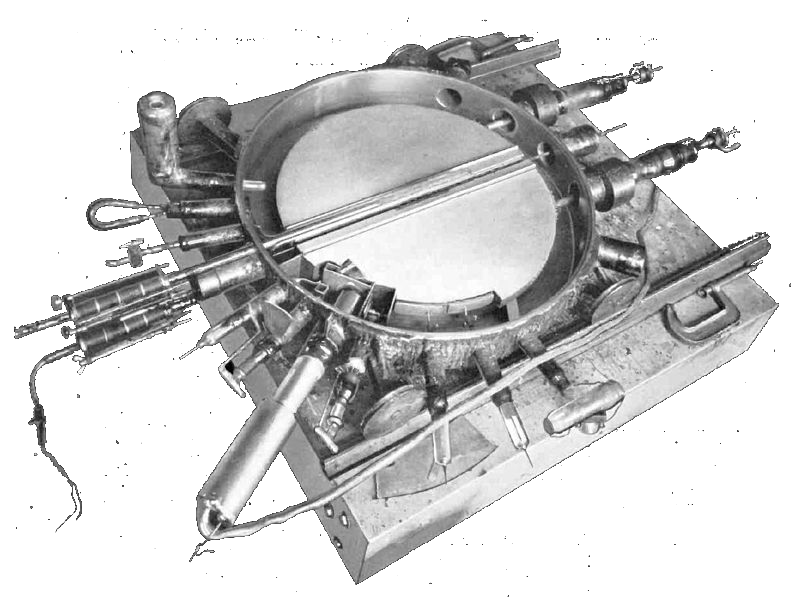
\includegraphics[width=\marginparwidth]{SM/cyclotron.png}
    \captionof{figure}{cyclotron de 27 pouces, accélérateur de $^{2}$H à 4 Mev (Université de Berkley, 1932).}
    	\label{atom}
}
\begin{figure}[h!]
\centering
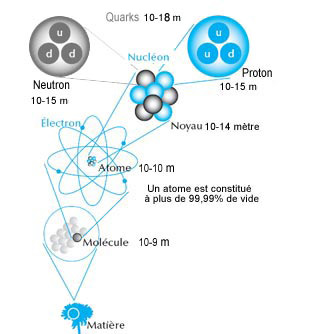
\includegraphics[width=0.50\textwidth]{SM/structure.jpg}
\captionof{figure}{Structure de la matière à différentes échelles.}
\label{structure}
\end{figure}

Parallèlement, de nouvelles interactions furent découverte. Elles expliquaient les désintégrations radiocatives ainsi que la cohésion des protons et des neutrons au sein du noyau atomique.

La physique des particules peut se résumer à la combinaisons des deux démarches précédentes, à savoir, trouver les particules élémentaires ainsi que de trouver les interactions fondamentales que ces particules peuvent subir. La manière dont ces particules interagissent aux moyens de ces interactions est donnée par la formulation mathématique d'une théorie, le Modèle Standard.

\subsection{Les particules élémentaires}
Les particules élémentaires du Modèle Standard, supposées indivisibles\footnote{à ce jour}, peuvent être classées en deux catégories selon leur spin (une propriété quantique intrasèque à chaque particule) :
\begin{itemize}[label=$\bullet$]
\item les \textit{fermions}, ils constituent la matières et sont de spin demi-entier.
\item les \textit{bosons}, ils sont les messagers de l'interaction et sont de spin entier.
\end{itemize}
Chaque particule du Modèle Standard possède des nombres quantiques telles que sa masse, sa charge électrique, en fraction de la charge électrique de l'électron e par convention (e=$1.6\times10^-19$ C). Dans le cadre de la théorie, à chaque particules correspond une anti-particule\footnote{Une particule peut être sa propre anti-particule.} qui possède la même masse mais dont les nombres quantiques sont opposés.

\subsubsection{Les fermions}
Les fermions peuvent être classés en deux catégories selon s'ils sont sensibles à l'interaction forte ou non. Dans le premier cas, ils font partis des \textit{quarks}, sinon ce sont des \textit{leptons}. Ces deux catégories sont elles-mêmes divisés en trois \textit{générations} \ref{fermions}.

Les leptons ont une charge électrique entière ($\pm$ 1) pour les électrons, muons et tau, et une charge nulle pour les neutrinos électronique, neutrinos muonique et neutrinos tauique.

Les quarks ont une charge électrique fractionnaire. On associe à chaque quark un nombre quantique appellé "couleur" (Rouge, Vert et Bleu). Dû à la propriètè de confinement de couleur, un quark ne peut être isolés et doivent se combiner avec un ou deux autre quarks afin de former des \textit{mésons} (fig.\ref{mésons}) et des \textit{baryons} (fig.\ref{baryons}) respectivement. La somme des deux (trois) couleurs des quarks doit constituer un mésons (baryon) "blanc" \footnote{Selon l'analogie avec la synthèse additive des couleurs.}. Les mésons et baryons sont regroupés sous le terme générique de \textit{hadrons}.
\marginpar
{
\hspace*{-0.5cm}
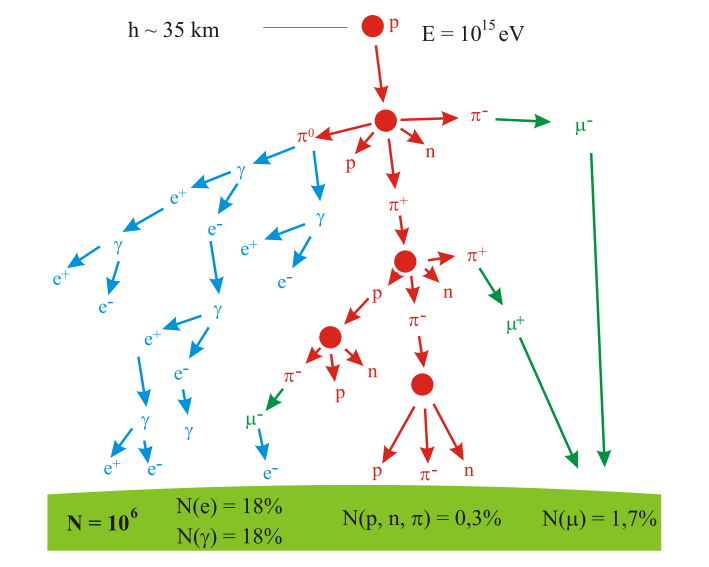
\includegraphics[width=1.2\marginparwidth]{SM/shower.png}
\captionof{figure}{Schéma d'une gerbe atmosphèrique.}
\label{gerbe}
}
\marginpar
{
	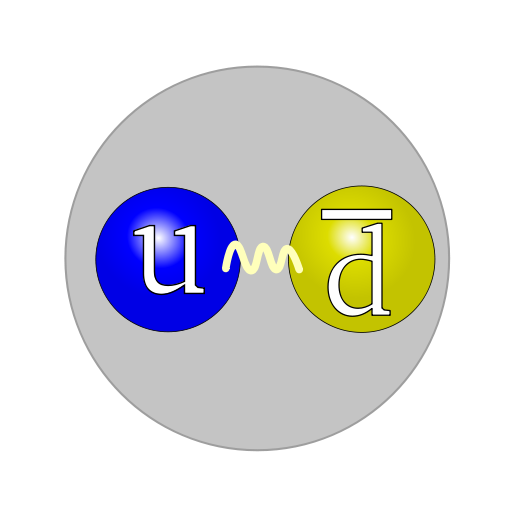
\includegraphics[width=\marginparwidth]{SM/quarks2.png}
    \captionof{figure}{Un méson ($\pi^{+}$).}
    	\label{mésons}
    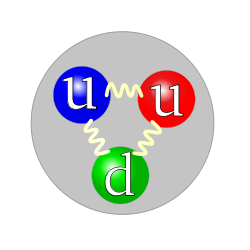
\includegraphics[width=\marginparwidth]{SM/quarks.png}
    \captionof{figure}{Un baryon ($p$).}
    	\label{baryons}
}
La matière qui nous entoure est composée que de particules de la première génération. Tous les atomes sont composés 'électrons et que quarks $u$ et $d$ qui s'assemblent pour donner des protons $p$ et neutrons $n$. Les autres particules peut être créer si l'énergie disponible est suffisante pour les créer (lors de gerbe atmosphérique où un proton vient interagir avec des particules de notre atmosphère par exemple \ref{gerbe} ou dans un collisionneur).
\definecolor{Orange}{HTML}{FFDD00}
\definecolor{Orange2}{HTML}{FFC000}
\definecolor{Green}{HTML}{8FB73E}
\definecolor{Green2}{HTML}{4EA700}
\definecolor{Red}{HTML}{EF4123}
\definecolor{Red2}{HTML}{EF2300}
\newcolumntype{P}[1]{>{\centering\arraybackslash}p{#1}}
\begin{table}[h!]
\centering
\begin{tabular}{|P{15mm}|P{39mm}|P{39mm}|P{39mm}|}
\hline 
\rowcolor{Orange2}Quarks & 1\iere génération & 2\ieme génération & 3\ieme génération \\
\hline 
\cellcolor{Orange2}\shortstack{ Nom \\ Notation \\  Charge  \\  Masse }&
\cellcolor{Orange}\shortstack{ Up \\ $u$,$\bar{u}$ \\ $\pm \frac{2}{3}$ \\ $0.005$ GeV/c$^2$} & 
\cellcolor{Orange}\shortstack{ Charm \\ $c$,$\bar{c}$ \\ $\pm \frac{2}{3}$ \\ $1.35$ GeV/c$^2$}&
\cellcolor{Orange}\shortstack{ Top \\ $t$,$\bar{t}$ \\ $\pm \frac{2}{3}$ \\ $172.6$ GeV/c$^2$}\\
\hline 
\cellcolor{Orange2}\shortstack{ Nom \\ Notation \\ Charge \\ Masse}& 
\cellcolor{Orange}\shortstack{ Down \\ $d$,$\bar{d}$ \\ $\mp \frac{1}{3}$ \\ $0.01$ GeV/c$^2$}& 
\cellcolor{Orange}\shortstack{ Strange \\ $s$,$\bar{s}$ \\ $\mp \frac{1}{3}$ \\ $0.1$ GeV/c$^2$}& 
\cellcolor{Orange}\shortstack{ Bottom \\ $b$,$\bar{b}$ \\ $\mp \frac{1}{3}$ \\ $1.3$ GeV/c$^2$}\\
\hline 
\rowcolor{Green2} Leptons & 1\iere génération & 2\ieme génération & 3\ieme génération \\
\hline
\cellcolor{Green2}\shortstack{ Nom \\ Notation \\ Charge \\ Masse}& 
\cellcolor{Green}\shortstack{ Électron \\ $e^{\pm}$ \\ $\pm 1$ \\ $0.511$ MeV/c$^2$}& 
\cellcolor{Green}\shortstack{ Muon \\ $\mu^{\pm}$ \\ $\pm 1$ \\ $105.7$ MeV/c$^2$}& 
\cellcolor{Green}\shortstack{ Tau \\ $\tau^{\pm}$ \\ $\pm 1$ \\ $1777$ MeV/c$^2$}\\
\hline 
\cellcolor{Green2}\shortstack{ Nom \\ Notation \\ Charge \\ Masse }& 
\cellcolor{Green}\shortstack{ Neutrino électronique \\ $\nu_{e}$ \\ $0$ \\ $<0.017$ MeV/c$^2$}& 
\cellcolor{Green}\shortstack{ Neutrino muonique \\ $\nu_{\mu}$ \\ $0$ \\ $<0.27$ MeV/c$^2$}&
\cellcolor{Green}\shortstack{ Neutrino tauique \\ $\nu_{\tau}$ \\ $0$ \\ $<35$ MeV/c$^2$}\\
\hline 
\end{tabular} 
\captionof{table}{Fermions: Quarks et Leptons.}
\label{fermions}
\end{table}

\subsubsection{Les bosons}
La description perturbative du Modèle Standard utilise l'échange de particules virtuelles, les bosons, afin de decrire l'interraction entre deux particules. Les bosons sont les médiateurs des interactions. Les particules de matière (fermions) interagissent donc entre elles par l'échange de particules de spin 1 correspondant à la force responsable de leur interaction.
\smallskip
Chacunes des quatres interactions possédent donc un ou plusieurs bosons appellés bosons de jauge (bosons vecteurs) (Tab.\ref{bosons}) :
\marginpar
{
\begin{center}
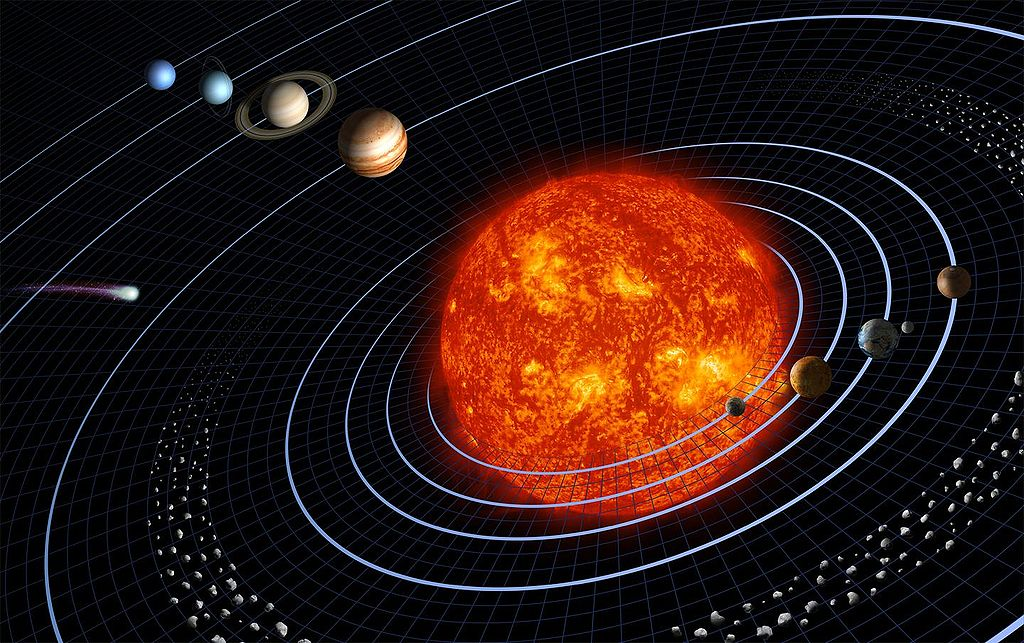
\includegraphics[width=\marginparwidth]{SM/solaire.jpg}
\begin{center}\normalfont\small {(a) Gravité : Système solaire.}\end{center}
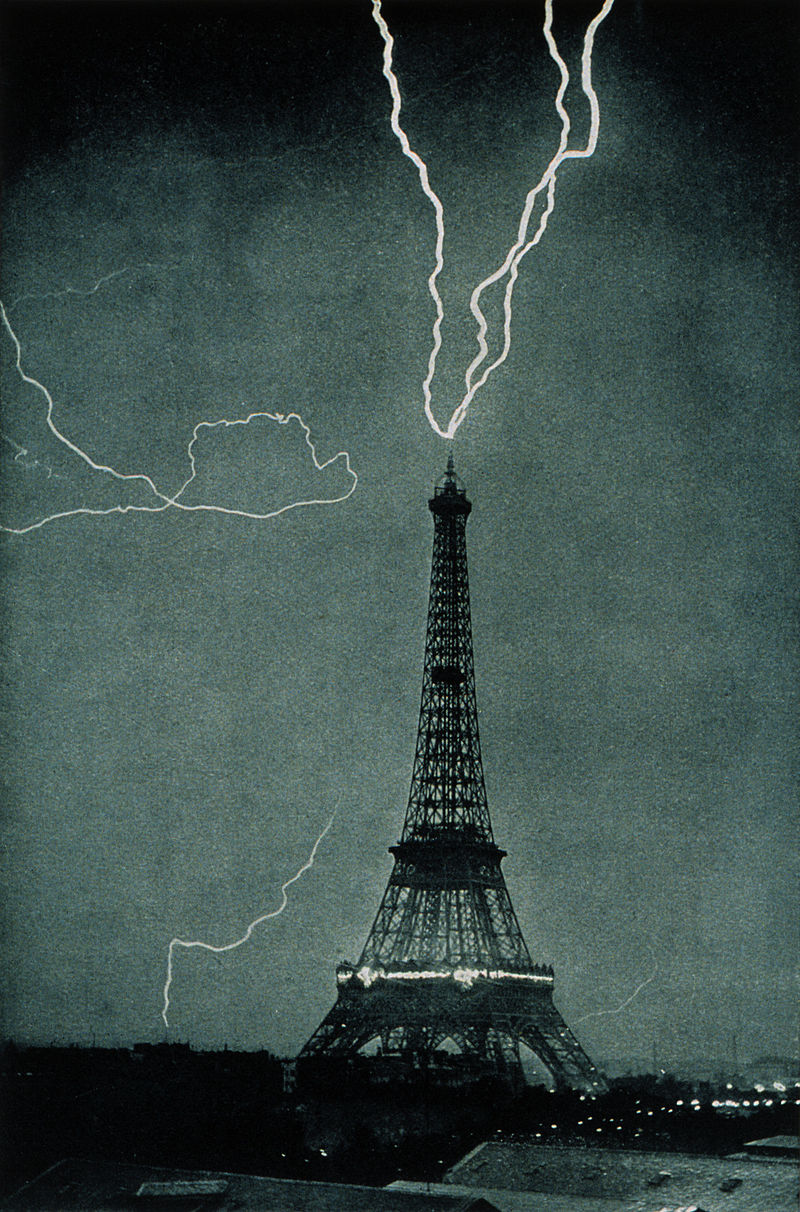
\includegraphics[width=\marginparwidth]{SM/foudre.jpg}
\begin{center}\normalfont\small {(b) Électromagnétisme : la foudre.}\end{center}
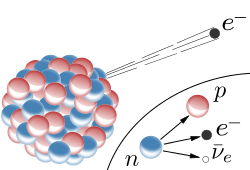
\includegraphics[width=\marginparwidth]{SM/beta.png}
\begin{center}\normalfont\small {(c) Interaction faible : désintégration $\beta$.}\end{center}
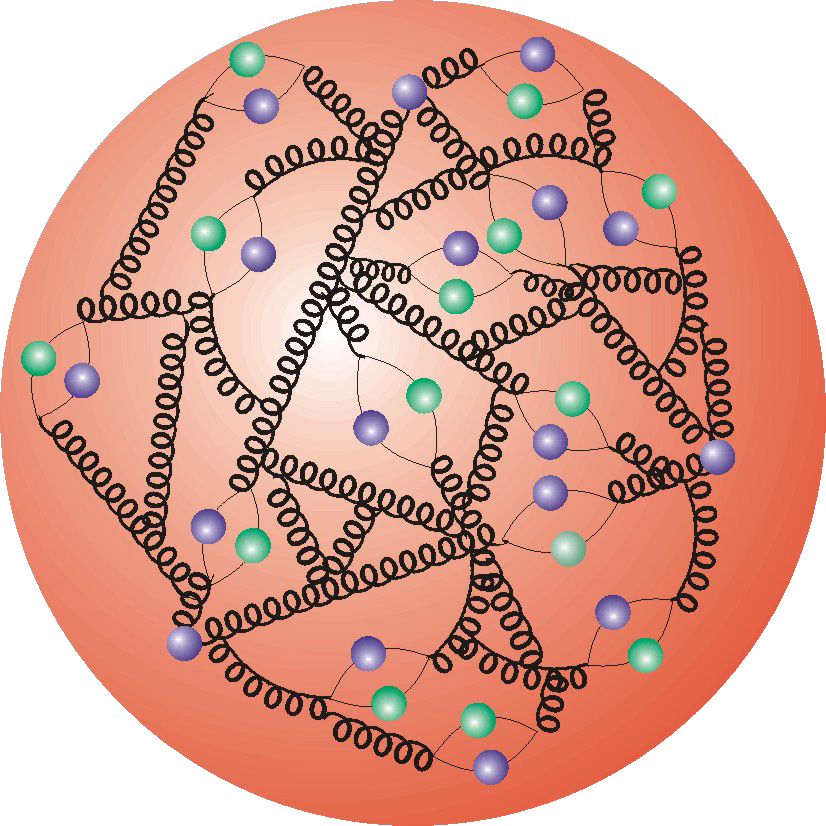
\includegraphics[width=0.8\marginparwidth]{SM/quarks3.png}
\begin{center}\normalfont\small {(d) Interaction forte : confinement.}\end{center}
\captionof{figure}{Exemple d'effets des 4 interactions.}
%\label{solides}
\end{center}
}
\begin{itemize}[label=$\bullet$]
\item \textbf{L'interaction gravitationnelle} est la première à avoir été découverte et expliquée (Galilée, Newton). Elle est négligeable à l'échelle atomique. Elle est gouverné par la masses des corps mises en jeu et elle domine à grande échelle ( Univers, Galaxies, Planètes, échelle humaine), son rayon d'action est infini. Son boson est encore activement recherché ( expériences Virgo et Ligo). Un pas décisif à été fait grâce à la détection par ces expériences des ondes Gravitationnelle. Cette interaction est la seule à ne pas être intégrée au Modèle Standard. Elle est actuellement décrite par la Relativité Générale qui est une approche non quantique.

\item \textbf{L'interaction électromagnétique} gouverne les interactions entre les particules chargées. C'est l'une des interactions qui nous ait la plus familière car elle est prépondérante dans notre vie quotidienne ( lumière, chimie, frottements ...). Tout comme la gravité, son rayon d'action est infinie. Son boson médiateur et le photon $\gamma$. C'est la seule interaction capable d'être attractive ou répulsive selon la charges des particules mises en jeu.

\item \textbf{L'interaction faible} à était découverte est comprise à travers la désintégration de particules avec changements de saveurs. Elle fait passer d'un fermion à un autre (par exemple lors de la désintégration $\beta$, elle transforme un neutron en un proton en chengeant un quark d en un quark $u$ et la crétaion d'un neutrino et d'un électron). Les bosons médiateurs de l'interaction sont les bosons $W^{+}$ $W^{-}$ $Z^{0}$. Sa portée est de l'ordre de 10$^{-18}$ m dû à la masse des bosons médiateur\footnote{Conséquence de l'incertitude de Heisenberg : $\Delta E \cdot \Delta t \geq \frac{\hbar}{2}$.}.

\item \textbf{L'interaction forte} permet l'échange de couleur entre les quarks et la création et l'annihilation de particules. Elle est résposable de la cohésion du noyau, et elle lie les nucléons entre eux à l'intérieur du noyau atomique. Ses bosons médiateur sont les gluons et sont au nombre de huit. Bien que les gluons soient supposés de masse nulle, la portée de l'interaction est de l'ordre de 10$^{-15}$ m. Cette portée est la conséquence du principe de confinement de couleur et à la liberté asymptotique qui affecte les quarks. En effet, cette interaction à la propriété de voir son interaction augmenter avec la distance, ce qui à tendance à regrouper les quarks entre eux. Cette propriètè est également responsable du processus d'hadronisation des quarks et de la création de jets.
\end{itemize}
\smallskip
\begin{table}[h!]
\centering
\begin{tabular}{|P{33mm}|P{26mm}|P{22mm}|P{52mm}|}
\hline 
\rowcolor{Red2}Interaction&Rayon d'action&Bosons de jauge&Masses\\
\hline 
\cellcolor{Red}\shortstack{ Forte }&
\cellcolor{Red}\shortstack{ $2.5\times10^{-15}$ m}& 
\cellcolor{Red}\shortstack{  Gluons (8)}&
\cellcolor{Red}\shortstack{ 0}\\
\hline 
\cellcolor{Red}\shortstack{ Electromagnétique }&
\cellcolor{Red}\shortstack{ $\infty$}& 
\cellcolor{Red}\shortstack{Photon $\gamma$}&
\cellcolor{Red}\shortstack{0}\\
\hline 
\cellcolor{Red}\shortstack{Faible}&
\cellcolor{Red}\shortstack{$10^{-18}$ m }& 
\cellcolor{Red}\shortstack{$W^{\pm}$,$Z^{0}$}&
\cellcolor{Red}\shortstack{$80.399$ Gev/c$^{2}$,$91.188$ Gev/c$^{2}$ }\\
\hline 
\cellcolor{Red}\shortstack{Gravitationnelle}&
\cellcolor{Red}\shortstack{$\infty$}& 
\cellcolor{Red}\shortstack{(Graviton)}&
\cellcolor{Red}\shortstack{(inconnue)}\\
\hline 
\end{tabular} 
\captionof{table}{Bosons : Interactions.}
\label{bosons}
\end{table}





 
    
  
 
 

